\par A técnica escolhida foi a Análise de Componentes Principais (em inglês, \textbf{Principal Component Analysis}). Além de ser uma das técnicas mais frequentemente utilizadas neste contexto, encontra-se disponível para uso em bibliotecas tais como o \textit{scikit-learn}.


\subsection{Análise de Componentes Principais (PCA)}

\par O PCA tem como objetivo preservar a maior quantidade de informação, fazendo
uma transformação de um vetor de $J$ elementos para um vetor de $I$ elementos
tal que $I \ll J$.
Assim, o número de dimensões a analisar pode ser reduzido sem que haja uma perda significativa de informação, pois o foco 
recai sobre a análise das dimensões principais que caracterizam o conjunto de dados.

\vspace{0.5em}

\par Para a aplicação desta técnica são necessários 5 passos:

\begin{itemize}
    \item Centrar na média;
    \item Cálculo da matriz de covariância;
    \item Cálculo dos valores e vetores próprios;
    \item Seleção do valor de redução;
    \item Projeção dos dados.
\end{itemize}

\vspace{0.5em}

\par O primeiro passo para o desenvolvimento desta técnica consiste numa \textbf{normalização} dos dados, isto é, subtrair a média de cada uma das dimensões que caracterizam o conjunto de dados, de modo a obter um novo conjunto, cuja a média é 0.

\vspace{0.5em}

\par De seguida é feito um cálculo da \textbf{matriz de covariância}. Esta relaciona a covariância entre todas as variáveis de um conjunto. Para esse efeito recorre-se à seguinte fórmula:

$$Cov = A^T \cdot A$$

\noindent Note-se que $A$ é a matriz com os dados de treino centrados na média, e $A^T$ a sua correspondente matriz transposta. 

\vspace{0.5em}

\par Numa fase seguinte, é feito o cálculo dos \textbf{valores e vetores próprios}. Estes representam as características principais de uma matriz. Serão calculados os valores e vetores próprios da matriz de covariância determinada anteriormente. Os \textbf{valores próprios} de uma certa matriz $A_{n \times n}$ são as raízes do polinómio característico de $A$. Esse calcula-se do seguinte modo:

$$ \Delta _ A(\lambda) = det (\lambda I - A )$$

\noindent Se $\lambda$ é valor próprio de $A$, então $(\lambda I -A) \cdot v = 0$ é um sistema possível indeterminado, ou seja, existe vetor $v \neq 0$ tal que: 

$$(\lambda I -A) \cdot v = 0$$

\noindent Para um valor próprio $ \lambda $, existe $ v \neq 0 $ tal que:

$$ Av = \lambda v $$

\noindent $v$ diz-se \textbf{vetor próprio} de $A$ associado a $ \lambda $.

\vspace{0.5em}

\par Posteriormente, é feita a \textbf{seleção do valor de redução}, ou seja, a escolha do número de componentes principais para reduzir. De modo a otimizar a escolha deste número, recorreu-se ao cálculo da variância explicada. Esta mede a proporção em que um modelo matemático é responsável pela variação de um determinado conjunto de dados.

\vspace{0.5em}

\par Recorreu-se ao \textbf{Python} para fazer um gráfico que relaciona a variância explicada cumulativa com diversos números de componentes principais. Este está ilustrado na Figura \ref{img1}.

\begin{figure}[H]
    \centering
    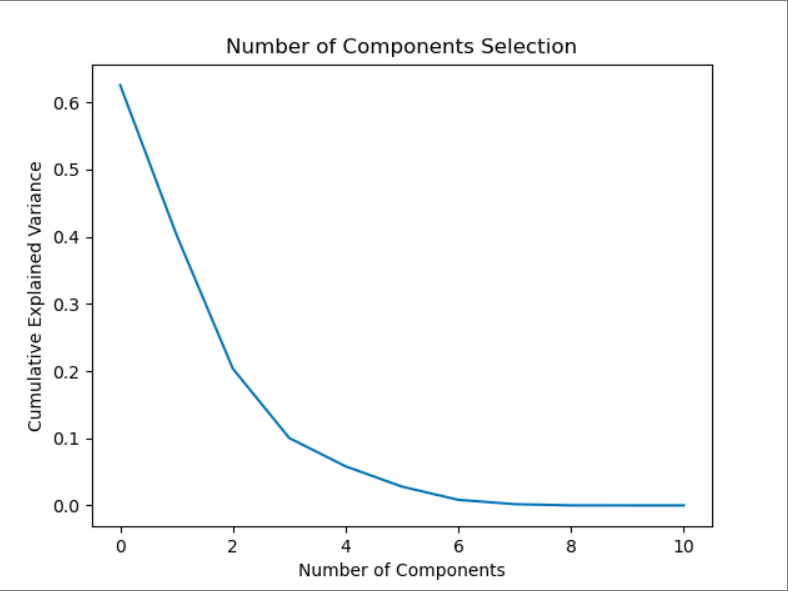
\includegraphics[width=\textwidth]{pca.png}
    \caption{Seleção do número de componentes}
    \label{img1}
\end{figure}


\noindent Pela análise da Figura \ref{img1}, aplicando a regra do cotovelo, conseguiu-se decidir o número de componentes, sendo este $K = 4$. 

\vspace{0.5em}

\par Por fim, é feita a \textbf{projeção dos dados}. Isto é conseguido através da multiplicação da matriz transposta que contém os vetores próprios resultantes da redução de dimensão, isto é, os mais relevantes, com a matriz transposta que contém os dados de treino centrados na média, ou seja, $V^T \cdot A^T$, sendo $V$ a matriz dos vetores próprios resultantes da redução de dimensão e $A$ a matriz com os dados de treino centrados na média. 